\subsection{Dolní a pásmová propust 2. řádu, 4. řádu}\label{s:DP2}
\noindent Obvodová simulace byla realizována v programu Multisim. Bylo zvoleno symetrické napájení (\textit{dual-supply}) $V_{DD},V_{SS} = \pm 15$ V. Pro symetrické napájení jsou výrobcem udávány hodnoty $V_{-} \in$ $[-16$ V ; -4.75 V] a $V_{+} \in$ $[4.75$ V ; 16 V]. Pro nesymetrické napájení (\textit{single-supply}) je doporučeno napájení $V_{+} \in$ $[9.5$ V ; 32 V]. Pokud by bylo cíleno na nižší napájecí napětí, bylo by to na úkor linearity, šumu, stejnosměrného zesílení v otevřených smyčkách a jednotkového zesílení šířky pásma, tzv. \textit{Unity Gain Bandwidth (UGBW)}, což je šířka pásma zesilovače při 0 dB (nezesiluje - jednotkové zesílení.\\
Regulací vstupního proudu je ovlivňován pracovní bod obvodu (mezní kmitočet). Vstupní externí proud $I_{ABC} = 0.5$ $\mu$A byl zvolen tak, aby byl obdržen mezní kmitočet cca 100 kHz. Maximální vstupní proud je 2 mA. Externím proudem $I_{ABC} \in$ $[5$ $\mu$A ; 500 $\mu$A] je garantováno minimální výstupní napětí $U_{OUT} = \pm 12$ V, standardně $V_{peak 1} = 14.2$ V a $V_{peak 2} = -14.4$ V. Při výstupním napětí v tomto intervalu je šum vzhledem k signálu zanedbatelný a nezkreslí výsledky simulace.\\
\noindent Diferenciální stupeň je podle literatury \cite{8} více či méně nelineární a lze tedy připustit maximální vstupní rozdílové napětí v řádech stovek mV. Překročení této meze vede k výraznému zkreslení signálu.\\
\noindent Bylo použito zapojení s paralelně řazeným uzemněným kapacitorem, odporem a indukčností (RLC rezonanční obvod), kde $R = 1/g_m$ a $L = C/(g_{m1}g_{m2})$ a vstupní proud $I = g_mV$. Podobně jako v sekci \ref{s:ODV} bylo obrženo analogií k pasivnímu obvodu
\begin{align}
\frac{V_{BP}}{g_{m3}V_i} &= \frac{1}{pC + g_m^2/(pC) + g_{m3}}\\
\frac{V_{BP}}{V_i} &= \frac{pg_{m3}C}{p^2C^2 + pg_{m3}C + g_m^2}.
\end{align}
\begin{figure}[h]
\centering
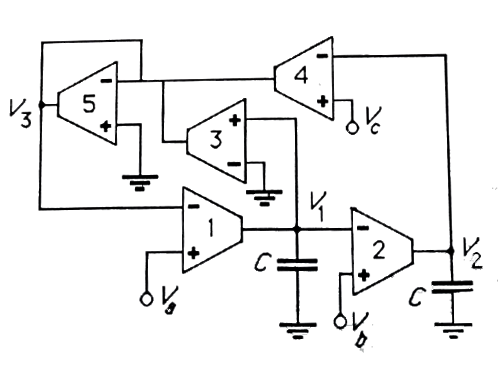
\includegraphics[scale=0.55]{biquad.png}
\caption[Obecná OTA struktura pro bikvad]{Obecná OTA struktura pro bikvad \cite{19} \label{s:BIK}}
\end{figure}
\begin{figure}[h]
\centering
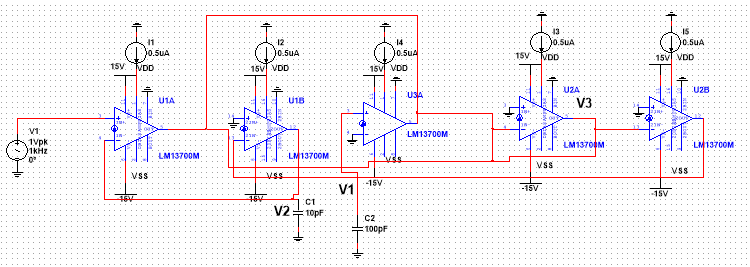
\includegraphics[scale=0.55]{bplphp.png}
\caption{Obecná OTA struktura pro bikvad - Multisim \label{s:BIK1}}
\end{figure}
\begin{figure}[h]
\centering
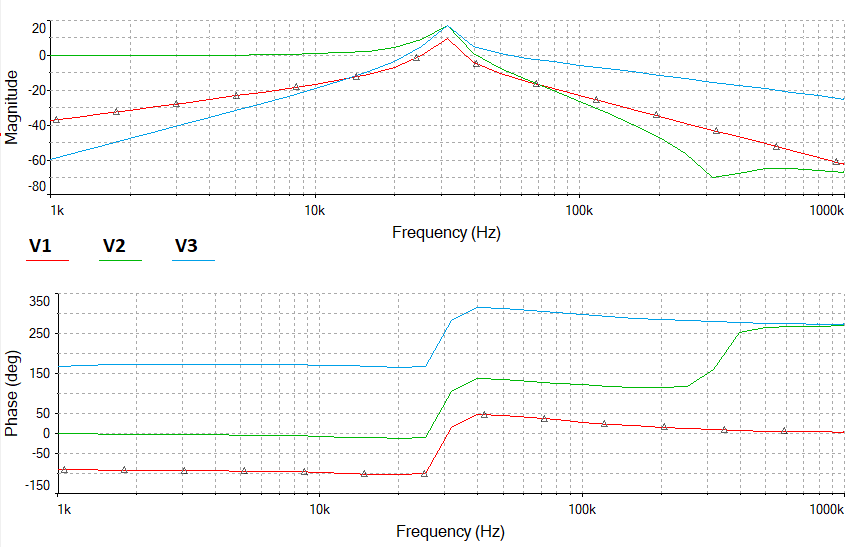
\includegraphics[scale=0.55]{bplphp2.png}
\caption{Obecná OTA struktura pro bikvad - Multisim \label{s:BIK2}}
\end{figure}
\noindent Zapojení podle literatury \cite{19} je popsáno na obrázku \ref{s:BIK}. Výstup z Multisimu lze vidět na obrázcích \ref{s:BIK1} a \ref{s:BIK2}. Uzlu označenému V1 odpovídá červený průběh (PP), uzlu V2 odpovídá modrý průběh (DP) a uzlu V3 zelený průbeh (HP). Zesilovače 1 a 2 na obrázku \ref{s:BIK} pracují jako invertující integrátory, zbývající zesilovače vytvářejí kladnou a zápornou zpětnou vazbu z výstupu integrátorů vedoucí na sčítací vstup. Znaménko vazby je určeno volbou vstupní svorky zesilovačů 3 a 4. Výstupy obvodu jsou napěťové (na výstupu sumačního zesilovače 5, resp. integrátoru 1 a 2). Buzení může být proudové (v obrázku \ref{s:BIK} na místě $V_1$ a $V_2$) nebo napěťové s využitím vstupních svorek transkonduktančních zesilovačů. Uvažováním napětí $V_a, V_b, V_c$ na obrázku \ref{s:BIK} jako vstupy byly obdrženy výstupní napětí
\begin{align}
V_1 &= \frac{pC_2g_{m1}(g_{m5}V_a - g_{m4}V_c) + g_{m1}g_{m2}g_{m4}V_b}{D(s)}\\
V_2 &= \frac{(pC_1g_{m2}g_{m5} + g_{m1}g_{m2}g_{m3})V_b + g_{m1}g_{m2}(g_{m4}V_c - g_{m5}V_a)}{D(s)}\\
V_3 &= \frac{p^2C_1C_2g_{m4}V_c + p(C_2g_{m1}g_{m3}V_a - C_1g_{m2}g_{m4}V_b) + g_{m1}g_{m2}g_{m4}V_a}{D(s)},
\end{align}\label{s:V3}
kde
\begin{equation}
D(p) = C_1C_2g_{m5}(p^2 + p\frac{1}{C_1}\frac{g_{m1}g_{m3}}{g_{m5}} + \frac{g_{m1}g_{m2}g_{m4}}{C_1C_2g_{m5}}).
\end{equation}\label{s:DS}
\noindent Zvolením $V_a = V_b = 0$ a $V_c = V_i$ byly obdrženy následující přenosové funkce
\begin{align}
H_{BP}(p) &= \frac{V_1}{V_i} = - \frac{sC_2g_{m1}g_{m4}}{D(s)}\\
H_{LP}(p) &= \frac{V_2}{V_i} = \frac{g_{m1}g_{m2}g_{m4}}{D(s)}\\
H_{HP}(p) &= \frac{V_3}{V_i} = \frac{s^2C_1C_2g_{m4}}{D(s)},
\end{align}
kde $D_s$ odpovídá rovnici \ref{s:DS}.\\
Obecná přenosová funkce bikvadu může být obdržena položením $V_a = V_b = V_c = V_i$ a úpravami vztahu \ref{s:V3} bylo obdrženo
\begin{equation}
\frac{V_3}{V_i} = \frac{p^2C_1C_2g_{m4} + p(C_2g_{m1}g_{m3} - C_1g_{m2}g_{m4}) + g_{m1}g_{m2}g_{m4}}{D(s)}.
\end{equation}
\noindent 
V simulaci byl dle výše popsaných poznatků na výstupu 2. OTA (V1) obdržen filtr typu PP 1. řádu s poklesem 20 dB/dek a na výstupu 3. OTA (V2) DP 2. řádu s poklesem 40 dB/dek. Mezní kmitočet pro dolní propust byl určen jako $88.359$ kHz - obrázek \ref{s:PET}. Šířka pásma pro pásmovou propust byla odečtena jako $48.291$ kHz. Změnou vstupního externího proudu (\textit{bias current}) na desetinu původní hodnoty, tedy $0.05 \mu$ A, došlo k posunutí mezního kmitočtu na $8.769$ kHz - obrázek \ref{s:PET1}. Šířka pásma u PP v tomto případě byla $4.779$ kHz.\\
\noindent Podle literatury \cite{10} lze v případě realizace těchto základních přenosů (PP, DP) zapojení dále zjednodušit až na obvod obsahující pouze 3 zesilovače, viz obrázek \ref{s:BIK2}. Toto zapojení však v simulaci neprokázalo dobré výsledky -- jednak docházelo k překmitu a jednak neměla pásmová propust symetrický průběh. Proto bylo zvoleno alternativní zapojení. Přenos obvodu z obrázku \ref{s:BIK2} s výstupem pořadě v bodu D a P je dán rovnicemi
\begin{align}
U_D(p) &= \frac{p\frac{g_{m3}U_3-g_{m2}U_2}{C_2}+\frac{g_{m1}g_{m2}}{C_1C_2}U_1}{p^2 + p\frac{g_{m3}}{C_2} + \frac{g_{m1}g_{m2}}{C_1C_2}}\\
U_P(p) &= \frac{p\frac{g_{m1}}{C_1}U_1 + \frac{g_{m1}}{C_1C_2}(g_{m3}U_1+g_{m2}-g_{m3}U_3)}{p^2 + p\frac{g_{m3}}{C_2} + \frac{g_{m1}g_{m2}}{C_1C_2}}.
\end{align}
\noindent Elementárními úpravami lze tyto rovnice zjednodušit na
\begin{align}
U_D(p) &= \frac{pC_1(g_{m3}U_3 - g_{m2}U_2) + g_{m1}g_{m2}U_1}{p^2C_1C_2 + pC_1g_{m3} + g_{m1}g_{m2}}\\
U_P(p) &= \frac{pC_2g_{m1}U_1 + g_{m1}(g_{m3}U_1 + g_{m2} - g_{m3}U_3)}{p^2C_1C_2 + pC_1g_{m3} + g_{m1}g_{m2}}.
\end{align}
\begin{figure}[h]
\centering
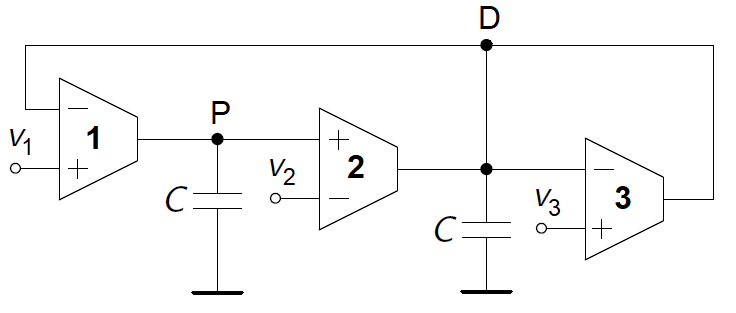
\includegraphics[scale=0.075]{biquad1.png}
\caption[Zjednodušená verze bikvadu OTA-C]{Zjednodušená verze bikvadu OTA-C \cite{10} \label{s:BIK2}}
\end{figure}
\noindent K sestavení dolní propusti 4. řádu bylo použito kaskádní zapojení sestávající ze sériově zapojených bloků. Přenosové funkce jednotlivých bloků se násobí
\begin{equation}
H_k(j\omega) = \frac{U_k (j\omega)}{U_{k-1}(j\omega)}.
\end{equation}
Přenos posledního bloku je dán vztahem
\begin{equation}
H_{1 \rightarrow k}(j\omega) = \frac{U_k (j\omega)}{U_{in}(j\omega)} = \prod _{n=1}^{k} H_n(j\omega).
\end{equation}
\begin{figure}[h]
\centering
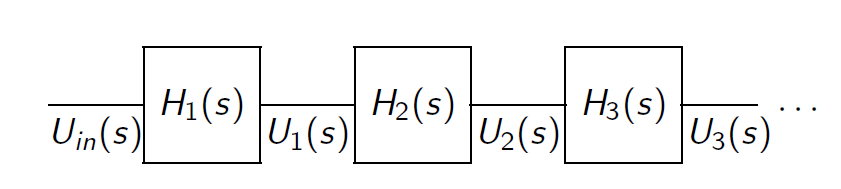
\includegraphics[scale=0.4]{schemata.png}
\caption[Kaskádní zapojení]{Kaskádní zapojení \cite{12}}
\end{figure}
Kaskádním zapojením dvou dolních propusti ze sekce \ref{s:DP2} byl obdržen filtr 4. řádu s poklesem 80 dB/dek a zároveň byla obdržena pásmová propust 2. řádu s poklesem 40 dB/dek. Mezní kmitočet pro dolní propust byl odečten jako 69.841 kHz. Šířka pásma pro PP byla 32.533 kHz. Výsledná napětí byla odebírána z uzlu V2 pro dolní propust a V1 pro pásmovou propust (obrázek \ref{s:DP4}). \\
\noindent Kaskádním zapojením dvou PP 2. řádu byla obdržena PP 4. řádu s poklesem 80 dB/dek. Šířka pásma byla odečtena jako 15.801 kHz.\\ Zapojení spočívá ve spojení dvou integrátorů, přičemž jeden z nich je neinvertující ztrátový a druhý invertující bezeztrátový. Výsledné napětí je odebíráno z uzlu V1 označeného na obrázku \ref{s:PP4}.\\
\noindent Přeladěním vstupního proudu na 3 $\mu$A byly pro ta samá zapojení obdrženy průběhy na obrázcích \ref{s:O1}, \ref{s:O2} a  \ref{s:O3}. Mezní kmitočet je pro DP 2. řádu 531.574 kHz a pro DP 4. řádu 420.012 kHz. Šířka pásma je pro PP 1. řádu 249.932 kHz, pro PP 2. řádu 202.051 kHz a pro PP 4. řádu 92.893 kHz.